\documentclass[addpoints,12pt]{exam}
%\documentclass[14pt]{exam}
\newcommand{\ds}{\displaystyle}
\usepackage[margin=0.8in]{geometry}
\usepackage{subcaption}
\usepackage{tikz}
\usepackage{amssymb,amsmath,graphicx,wrapfig,verbatim, psfragx,color}
\usepackage{multicol}
\usepackage{wasysym}
\def\FillInBlank{\rule{3truein} {.01truein}}
% Choose one option (bubbles)
\newcommand{\chooseone}{{\Large$\Circle$\ \ }}
\usepackage{amssymb,amsmath,graphicx,wrapfig,verbatim, psfragx,color}
\usepackage{multicol}
% If you want them as a list (instead of next to each other)
\usepackage{enumitem}
% ---- Convenience commands -----
% Choose one option (bubbles)
%\newcommand{\chooseone}{{\Large$\Circle$\ \ }}
% ---- Example Usage | Multiple Choice -----
%\usepackage{fancyhdr}
%\setlength{\headheight}{13.6pt}
%\pagestyle{fancy}
%\lhead{Math 222}
%\chead{ Midterm 1 }
%\rhead{Spring 2022}
\def\FillInBlank{\rule{3truein} {.01truein}}
\newcommand{\TorF}{\hspace{.1in} \textbf{True} \hspace{.1in} \textbf{False} \hspace{.1in}}
\begin{document}
\begin{enumerate}
\item Let $\vec{a} = \langle 2, 1, -3 \rangle$ and $\vec{b} = \langle 4, -1, -2 \rangle.$
\begin{itemize}
\item[4] Find a vector of length $2$ that points in the opposite direction of $\vec{a}.$
\vfill
\item[8] Find the area of the parallelogram spanned by $\vec{a}$ and $\vec{b}.$
\vfill
\vfill
\end{itemize}
\newpage
\item[5] Find the equation of a line that is perpendicular to the plane $2x -3y+7z = 12$ and
that contains the point $(8, 9, -2).$
\vfill
\item[10] Find an equation for the plane that contains the points $A = (2,-1,3),$ $B = (1, 2,
-1)$ and $C = (0, 4, 3).$
\vfill
\vfill
\vfill
\newpage
\item Consider the figure shown. In this picture, $P = (1,0,0)$, $Q = (1,6,0)$, and $R =
(2,4,3)$.
\begin{itemize}
\item[1] Compute the vector $\overrightarrow{PR}$. Write your answer in the provided answer
box.
\vfill
\begin{flushright}
\fbox{\parbox{.35\textwidth}{\hspace{1.5in}\\
$ \rm{\overrightarrow{PR} = } $\hspace{.7in} \\}}
\end{flushright}
\item[1] Compute the vector $\overrightarrow{PQ}$. Write your answer in the provided answer
box.
\vfill
\begin{flushright}
\fbox{\parbox{.35\textwidth}{\hspace{1.5in}\\
$ \rm{\overrightarrow{PQ} = } $\hspace{.7in} \\}}
\end{flushright}
\item[5] Compute the vector $\overrightarrow{PM}$ (that is, compute the projection of the vector
$\overrightarrow{PR}$ onto the vector $\overrightarrow{PQ}$). Write your answer in the
provided answer box. You WILL be graded for your work, so make sure to justify your answer.
\vfill
\vfill
\vfill
\vspace{0.1in}
\begin{flushright}
\fbox{\parbox{.35\textwidth}{\hspace{1.5in}\\
$ \rm{\overrightarrow{PM} = } $\hspace{.7in} \\}}
\end{flushright}
\item[2] Compute the vector $\overrightarrow{MR}$. Write your answer in the provided answer
box. You WILL be graded for your work, so make sure to justify your answer.
\vfill
\vfill
\vspace{0.1in}
\begin{flushright}
\fbox{\parbox{.35\textwidth}{\hspace{1.5in}\\
$ \rm{\overrightarrow{MR} = } $\hspace{.7in} \\}}
\end{flushright}
\end{itemize}
\newpage
\item Consider the surface $y =x^2 + 9z^2$.
\begin{itemize}
\item[4] Sketch the traces in the vertical planes $x = k$, with $ k =0, 1$. Label your traces.
\begin{center}
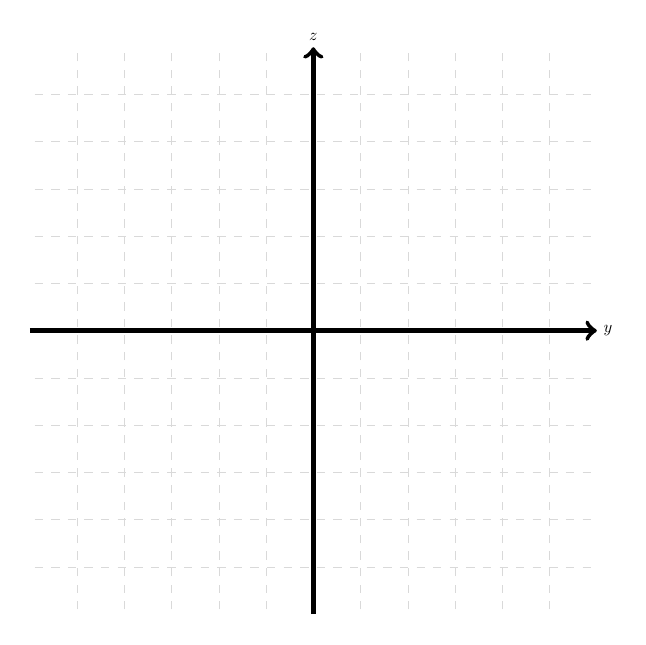
\begin{tikzpicture}[scale=0.6, transform shape]
\draw[help lines, color=gray!30, dashed] (-5.9,-5.9) grid (5.9,5.9);
\draw[->,ultra thick] (-6,0)--(6,0) node[right]{$y$};
\draw[->,ultra thick] (0,-6)--(0,6) node[above]{$z$};
\end{tikzpicture}
\end{center}
\vfill
\item[4] Sketch the traces in the vertical planes $y = k$, with $ k =0, 1 $. Label your traces.
\begin{center}
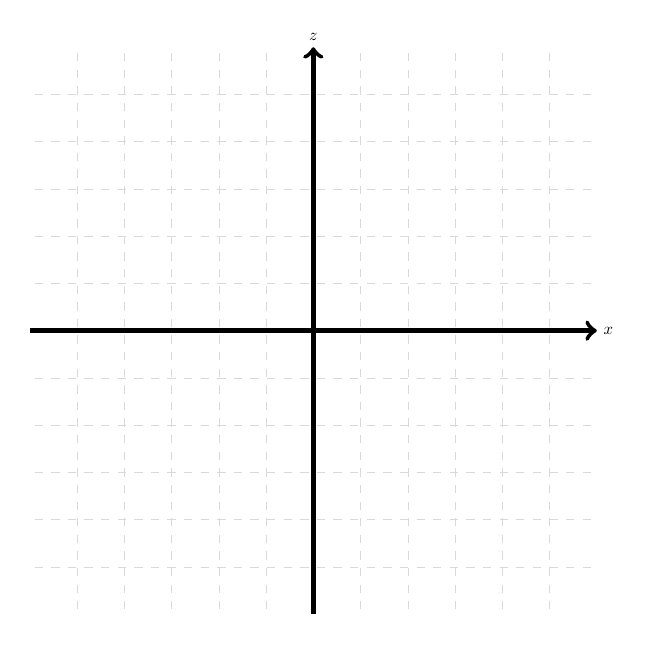
\begin{tikzpicture}[scale=0.6, transform shape]
\draw[help lines, color=gray!30, dashed] (-5.9,-5.9) grid (5.9,5.9);
\draw[->,ultra thick] (-6,0)--(6,0) node[right]{$x$};
\draw[->,ultra thick] (0,-6)--(0,6) node[above]{$z$};
\end{tikzpicture}
\end{center}
\vfill
\end{itemize}
\newpage
\item Consider the curve $\vec{r}(t) = \langle 3t-2, \cos(\pi t), t^2 +1 \rangle.$
\begin{itemize}
\item[5] Write down an integral that represents the length of the curve from the point $(4, 1, 5)$
to the point $(7, -1, 10).$ You do NOT need to compute the integral.
\vfill
\item[4] Find an equation for the tangent line to the curve at the point $(4, 1, 5).$
\vfill
\end{itemize}
\newpage
\item[8] Consider the surfaces $ z = 2x+2$ and $ z = x^2+y^2-1.$ Find a vector function
that represents the curve of intersection of the given surfaces.
\newpage
\item Consider the curve given by $\vec{r}(t)=\langle 3\cos(t),4t,5-3\sin(t)\rangle$
\begin{itemize}
\item[6] Find the unit tangent vector, $\vec{T}(t).$
\vfill
\item[6] Find the unit normal vector, $\vec{N}(t).$
\vfill
\item[4] Find the curvature, $\kappa(t).$
\vfill
\end{itemize}
\newpage
\item[8] An object's velocity is given by
$$\vec{v}(t) = \langle 6t^2+5, 2+ 3\sqrt{t} , 4e^{2t} \rangle.$$
Its initial position is $\vec{r}(0) = \langle 2,\pi,0 \rangle.$ Find a vector equation $\vec{r}(t)$ for
the position of the object at time $t.$
%\item[6] Find a vector equation $\vec{r}(t)$ for the position of the object at time $t.$
\newpage
\item Consider the function $f(x,y) = \dfrac{\sqrt{x-y}}{ \ln(2+ x^2 +y^2)}.$
\begin{itemize}
\item[2] Find the domain of the function.
\vfill
\item[4] Sketch the domain of the function. Shade the region(s) that are part of the domain. Use
dotted lines when sketching a curve that is NOT in the domain, and solid lines when sketching
curves that are.
\vfill
\vfill
\end{itemize}
\newpage
\item[9] If the limit exists, compute it (making sure to justify your answer). If the limit does
not exist, justify why it doesn’t exist. If you use a theorem, state clearly which theorem you are
using. Make sure to use correct limit notation.
$$\displaystyle\lim_{(x,y) \to (0,0)} \dfrac{4xy^3}{2x^4 + 3y^4}$$
\vfill
\newpage
\end{enumerate}
\end{document}
